\paragraph{Brio \& Wu Shock Tube}

The Brio \& Wu Shock Tube \citep{brio_wu_1988} is a staple test of MHD codes. This Riemann problem is essentially the Sod shock tube \citep{sod_1978} with a magnetic field. However, this shock tube is an excellent stress test for PPM reconstruction, as methods higher than second order tend to create large oscillations in the solution due to the slowly moving shock waves. We have implemented both the PPM reconstruction algorithm used in the VL+CT integrator from the method described in \cite{stone_athena_2008} as well as the method described in \cite{felker_2018}, and find that the latter significantly reduces oscillations for this test. With PPM reconstruction, we find  oscillations in the solution when limiting in either the primitive or characteristic variables. No oscillations are present when using PLM reconstruction.

\begin{figure}[ht!]
    % \epsscale{0.5}
    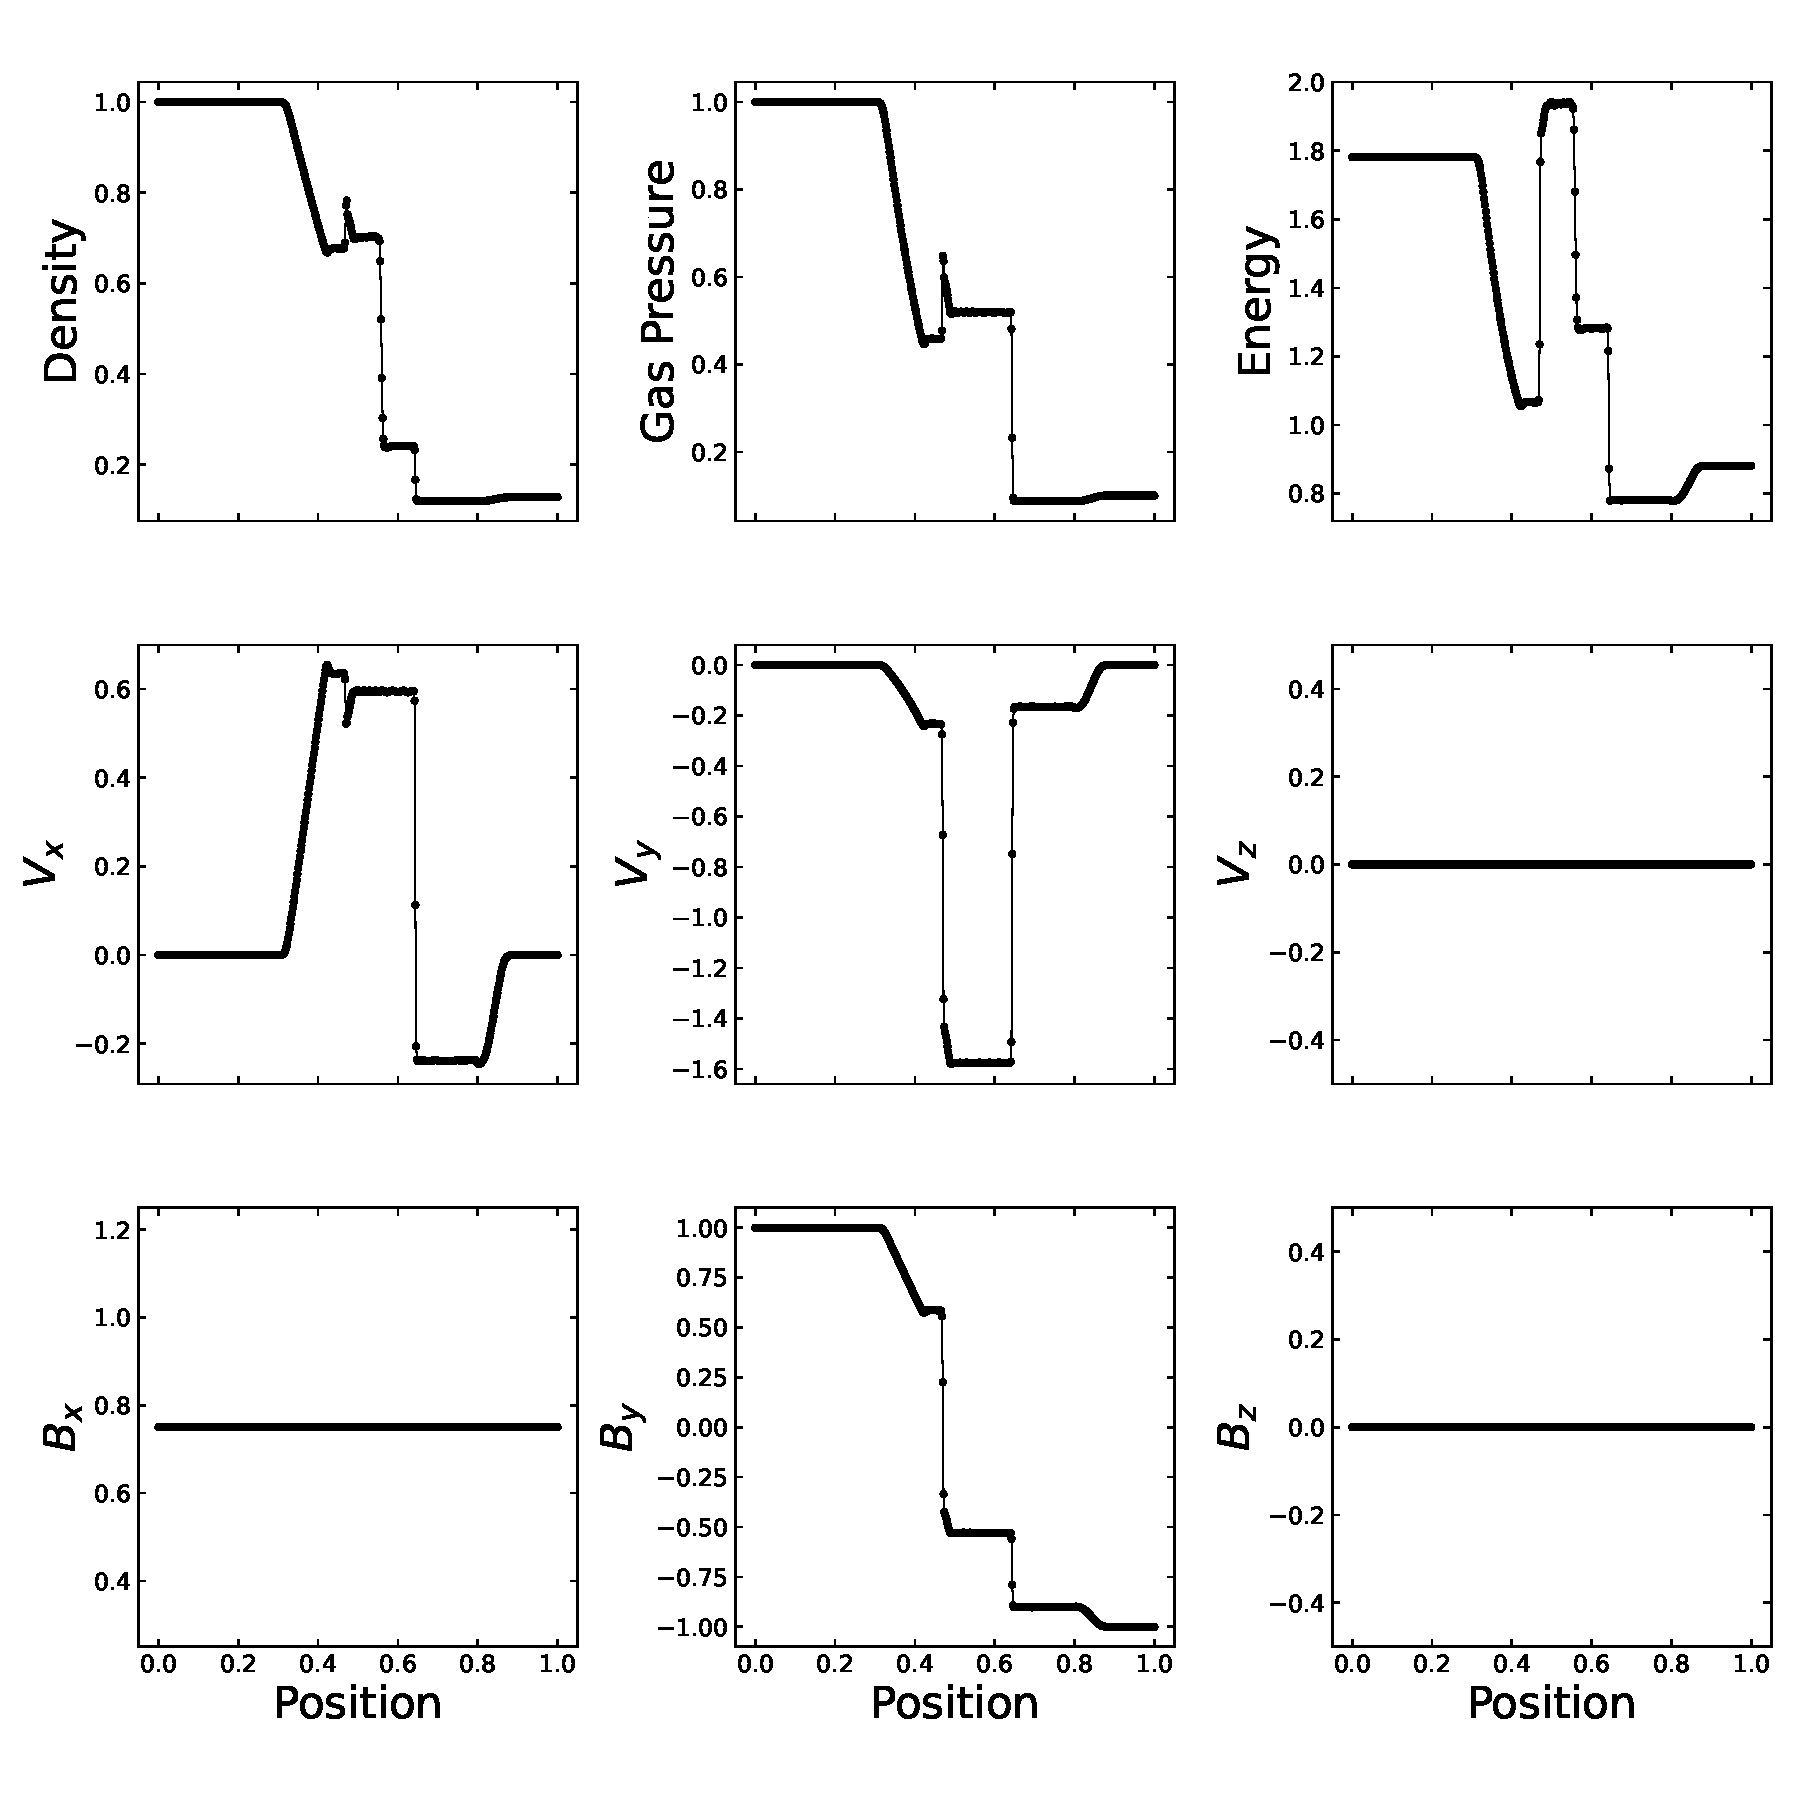
\includegraphics[width=\linewidth]{assets/3-mhd-tests/b&w.pdf}
    \caption{The Brio \& Wu Shock Tube solution \citep{brio_wu_1988}.
    \input{|python ../python/get_links.py 'b&w'}}
    \label{fig:brio-and-wu}
\end{figure}

\paragraph{Dai \& Woodward Shock Tube}

The Dai \& Woodward Shock Tube (also called Ryu \& Jones 2a) \citep{dai_woodward_1998, ryu_jones_1995} produces all seven possible MHD waves. From left to right they are: fast shock, Alfvén wave, slow shock, contact discontinuity, slow shock, Alfvén wave, and fast shock. This makes it an excellent laboratory for checking that the full spread of wave modes are well resolved.

\begin{figure}[ht!]
    % \epsscale{0.5}
    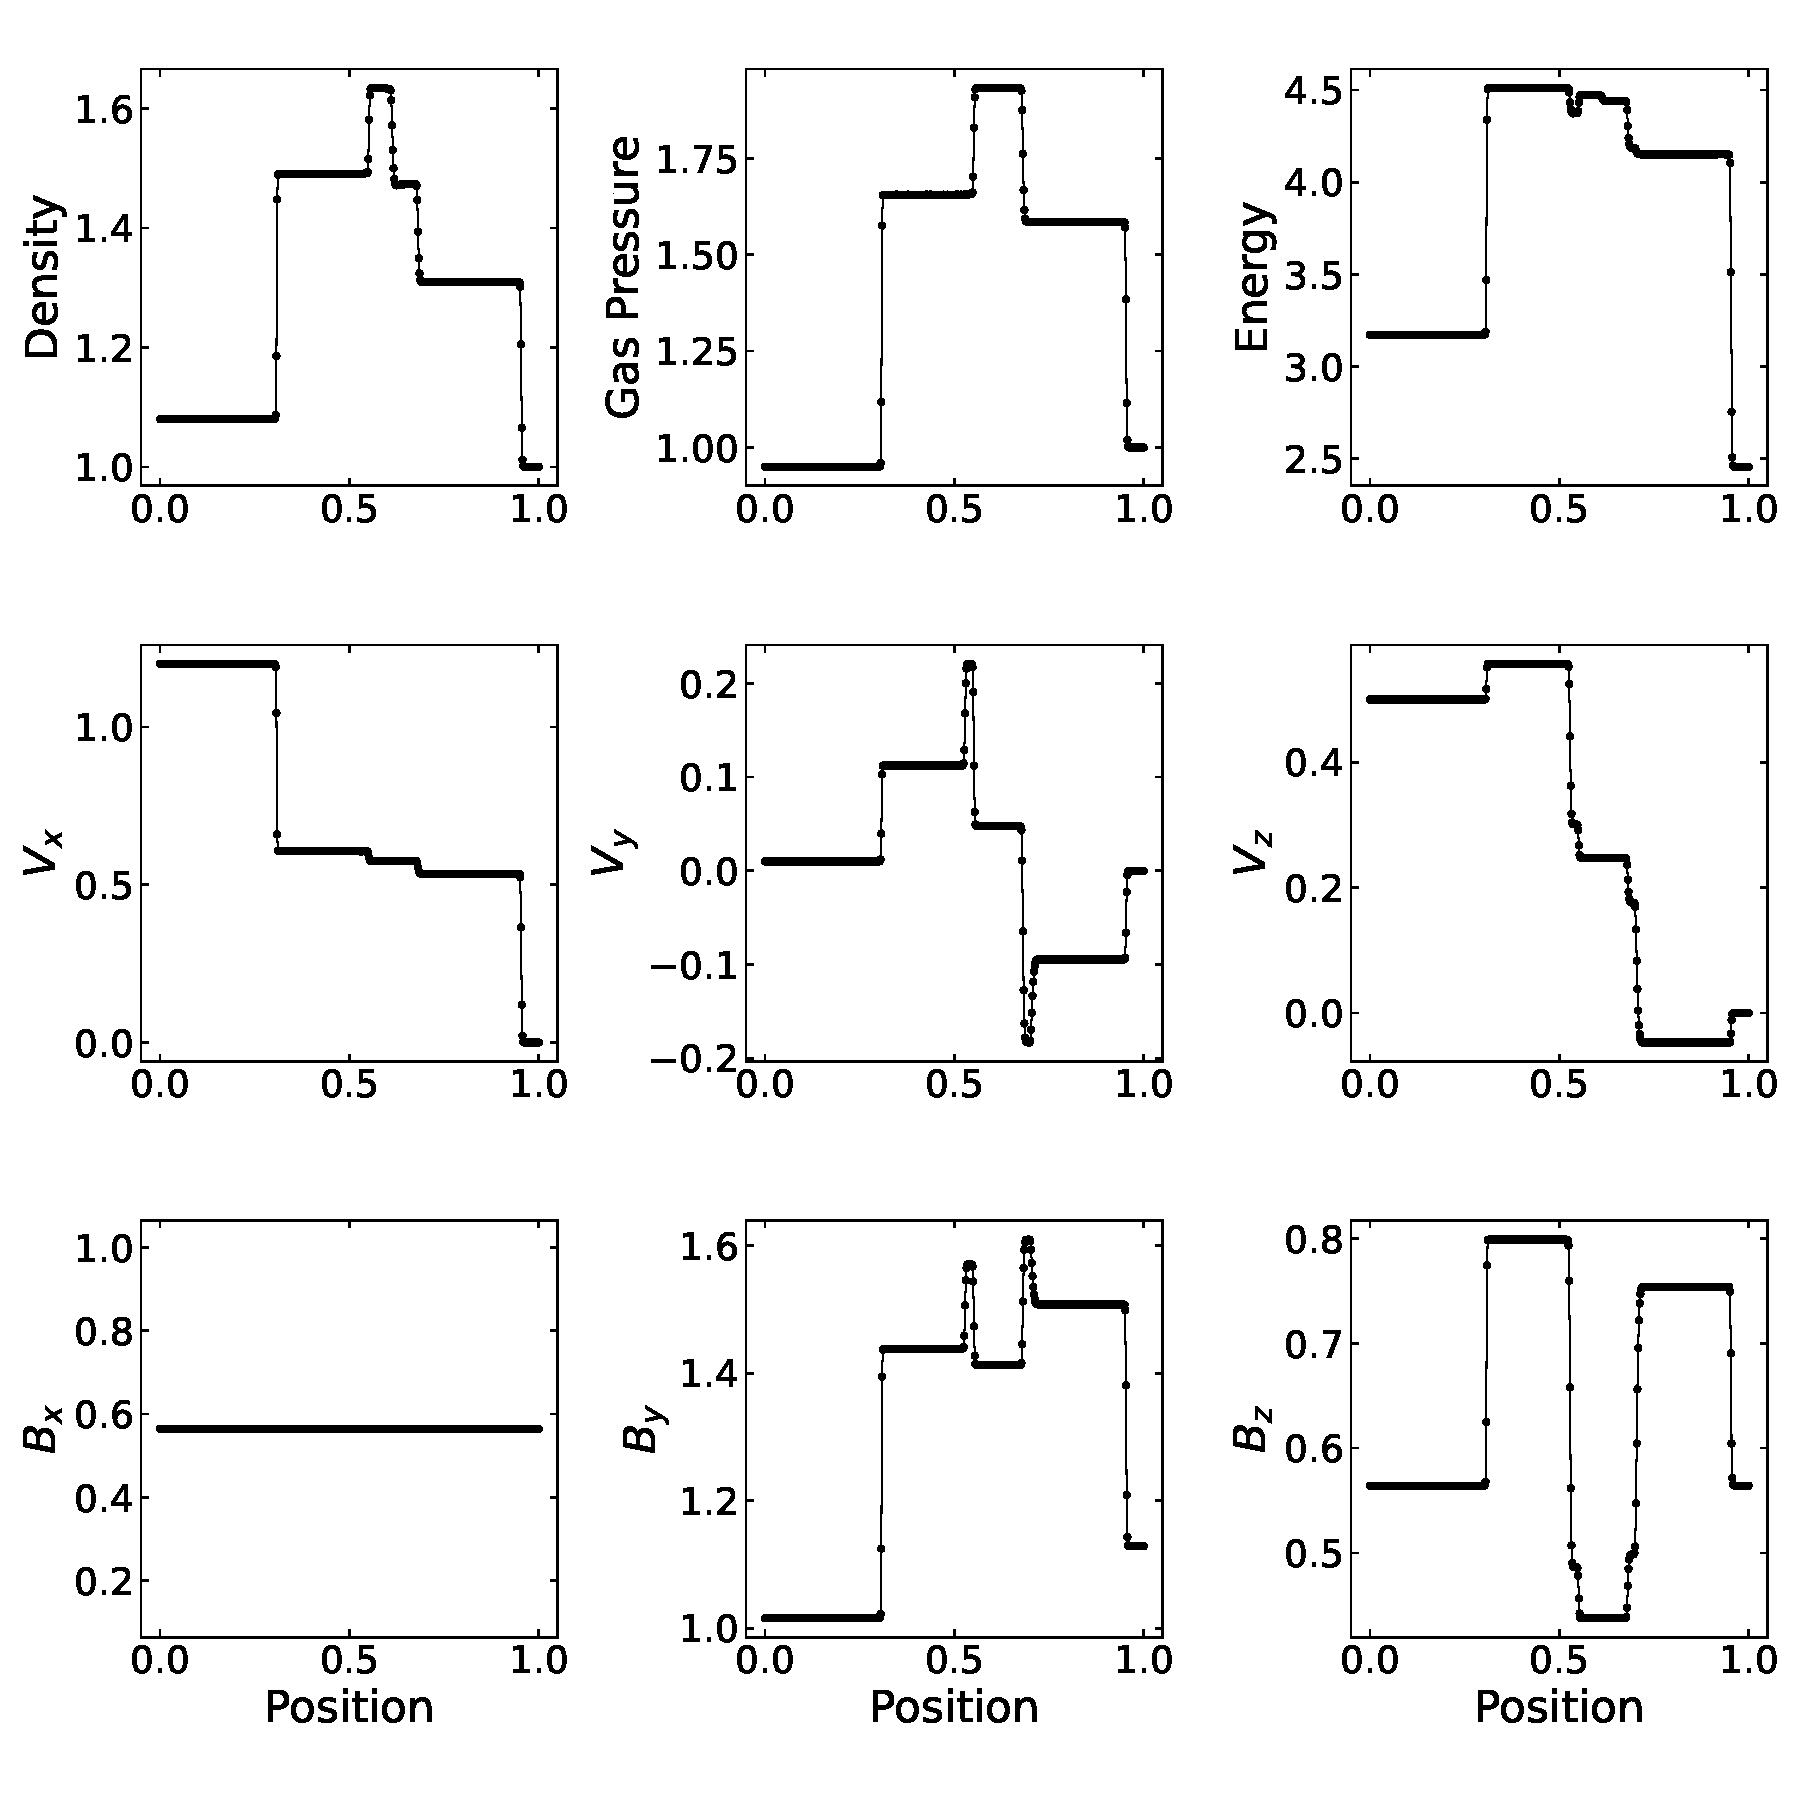
\includegraphics[width=\linewidth]{assets/3-mhd-tests/d&w.pdf}
    \caption{Dai \& Woodward Shock Tube (also called Ryu \& Jones 2a) solution \citep{dai_woodward_1998, ryu_jones_1995}.
    \input{|python ../python/get_links.py 'd&w'}}
    \label{fig:dai-and-woodward}
\end{figure}

\paragraph{Ryu \& Jones 1a Shock Tube}

Ryu \& Jones 1a Shock Tube solution \citep{ryu_jones_1995} is a less common test for MHD codes. However, in our experience, it is an excellent problem for debugging due to its relatively simple structure, which doesn't contain any of the large spikes present in other tests, that are difficult to discern by eye during the evolution of the initial conditions. The lack of any spikes and the presence of multiple types of strong shocks also make it a good diagnostic test for over/undershoot of the solution near discontinuities.

\begin{figure}[ht!]
    % \epsscale{0.5}
    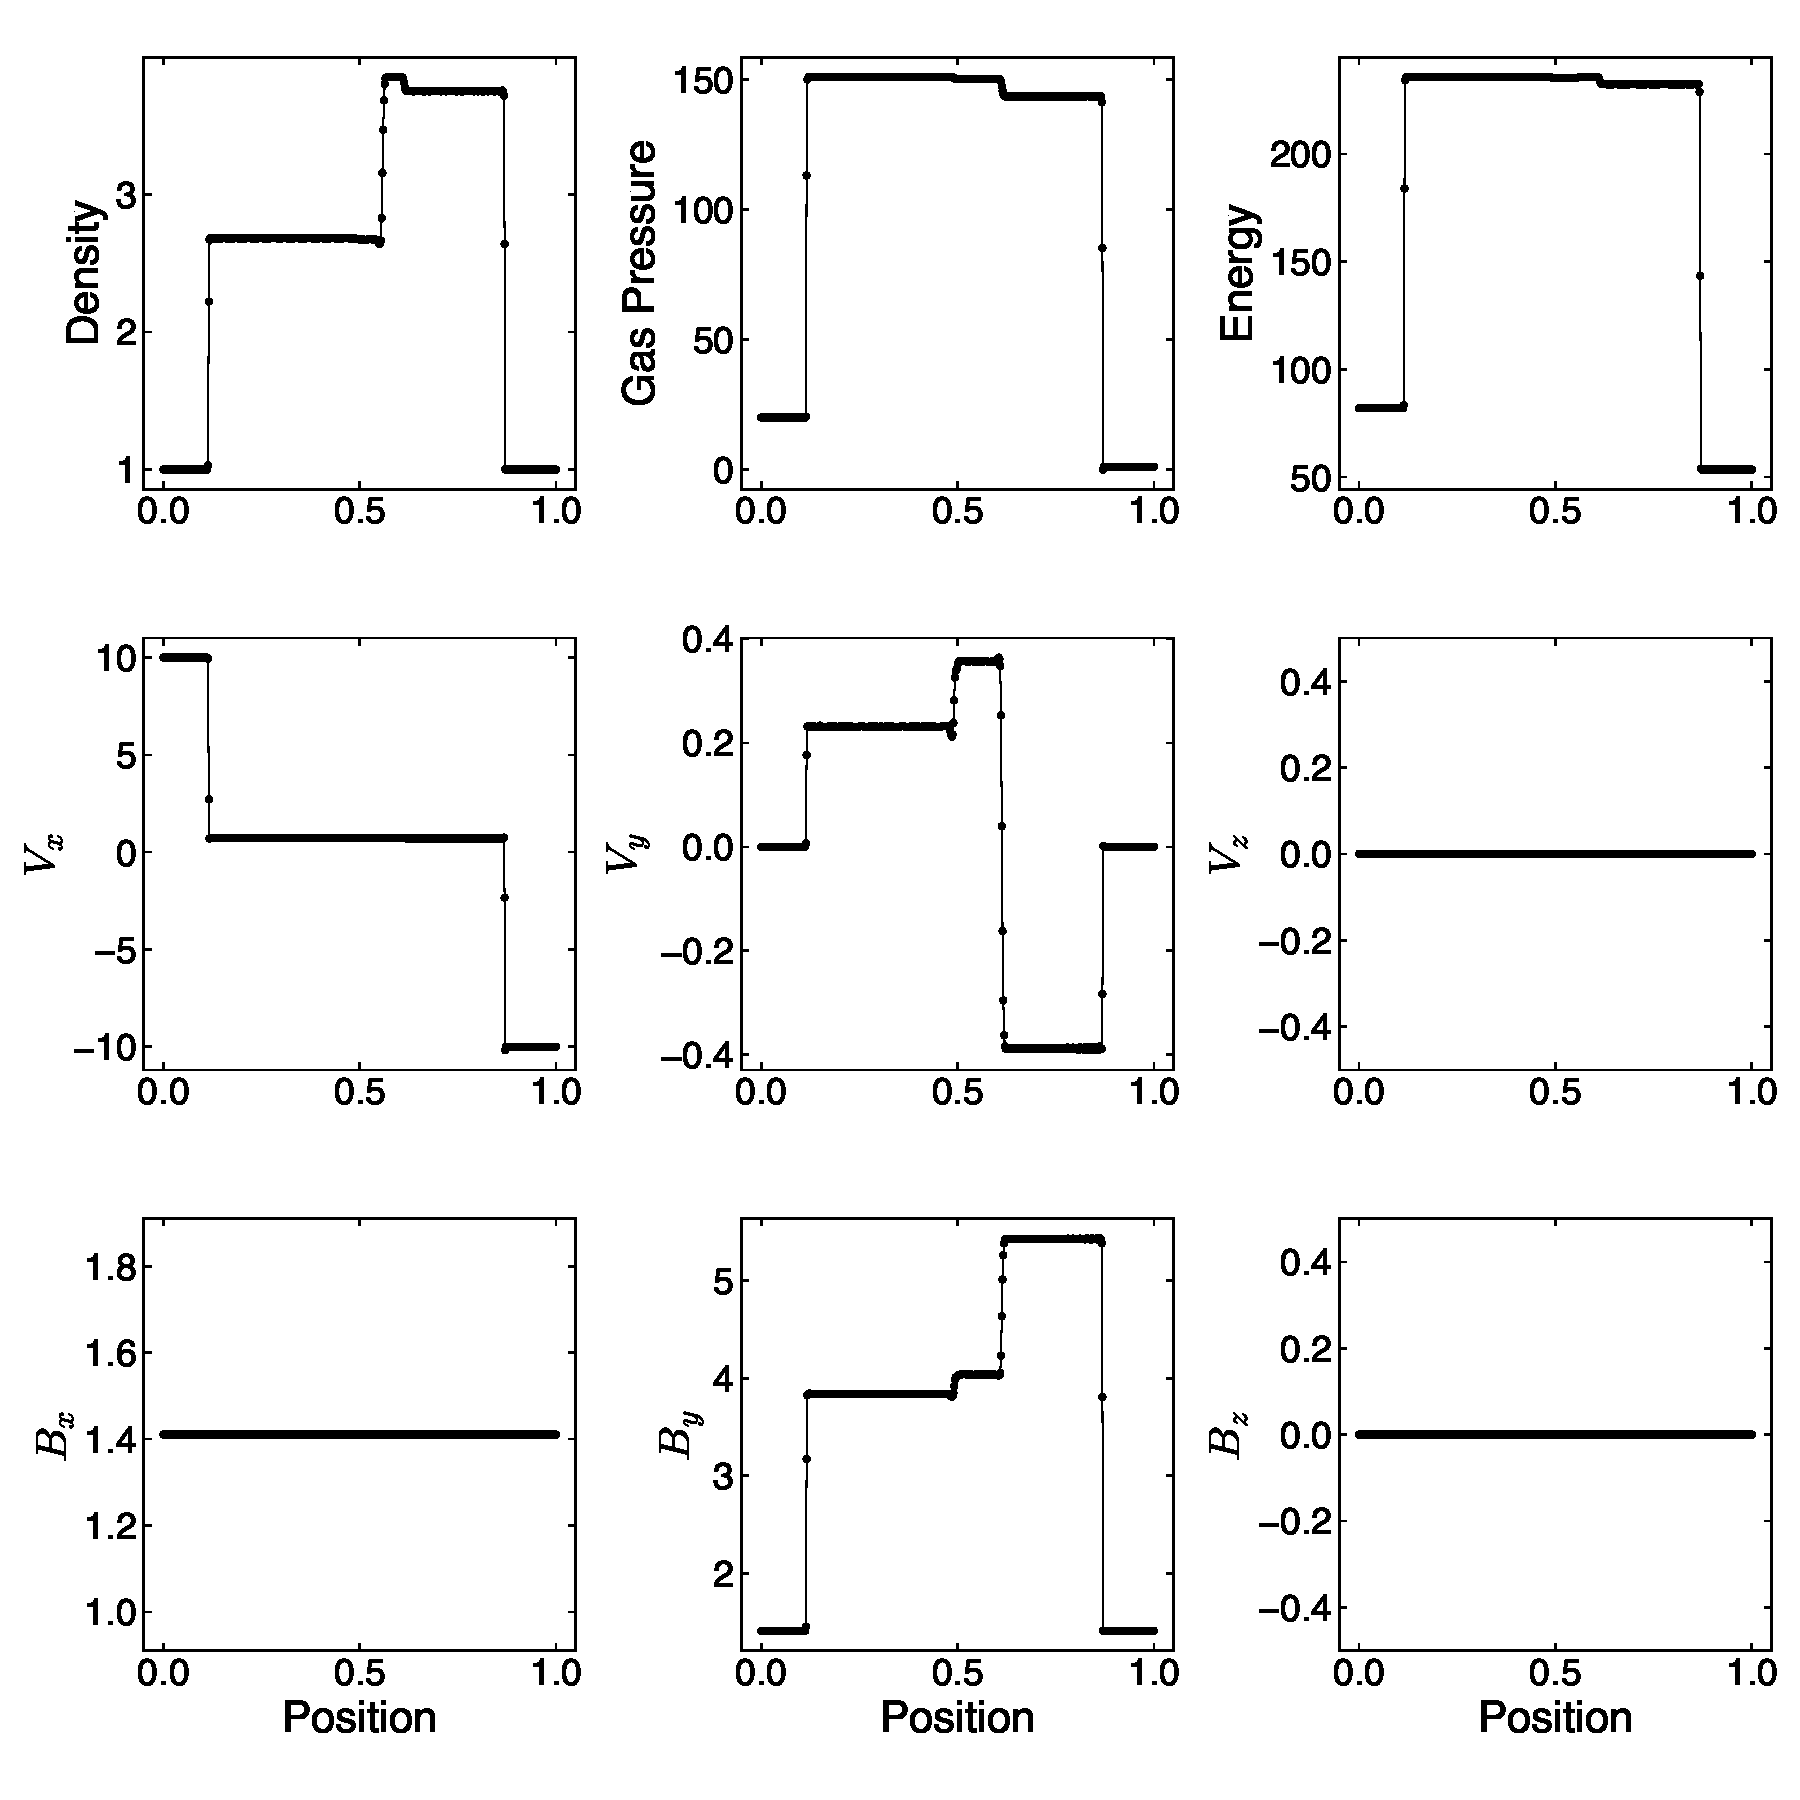
\includegraphics[width=\linewidth]{assets/3-mhd-tests/rj1a.pdf}
    \caption{Ryu \& Jones 1a Shock Tube solution \citep{ryu_jones_1995}.
    \input{|python ../python/get_links.py 'rj1a'}}
    \label{fig:rj-1a}
\end{figure}

\paragraph{Ryu \& Jones 4d Shock Tube}

The Ryu \& Jones 4d Shock Tube solution \citep{ryu_jones_1995} features a switch-on slow shock. Switch-on waves increase the strength of the transverse magnetic field while reducing the thermal pressure to maintain energy conservation. This is a simplified example of a type of magnetic field amplification and as such it is important to demonstrate that a code can replicate it accurately. A switch-off wave does the inverse.

\begin{figure}[ht!]
    % \epsscale{0.5}
    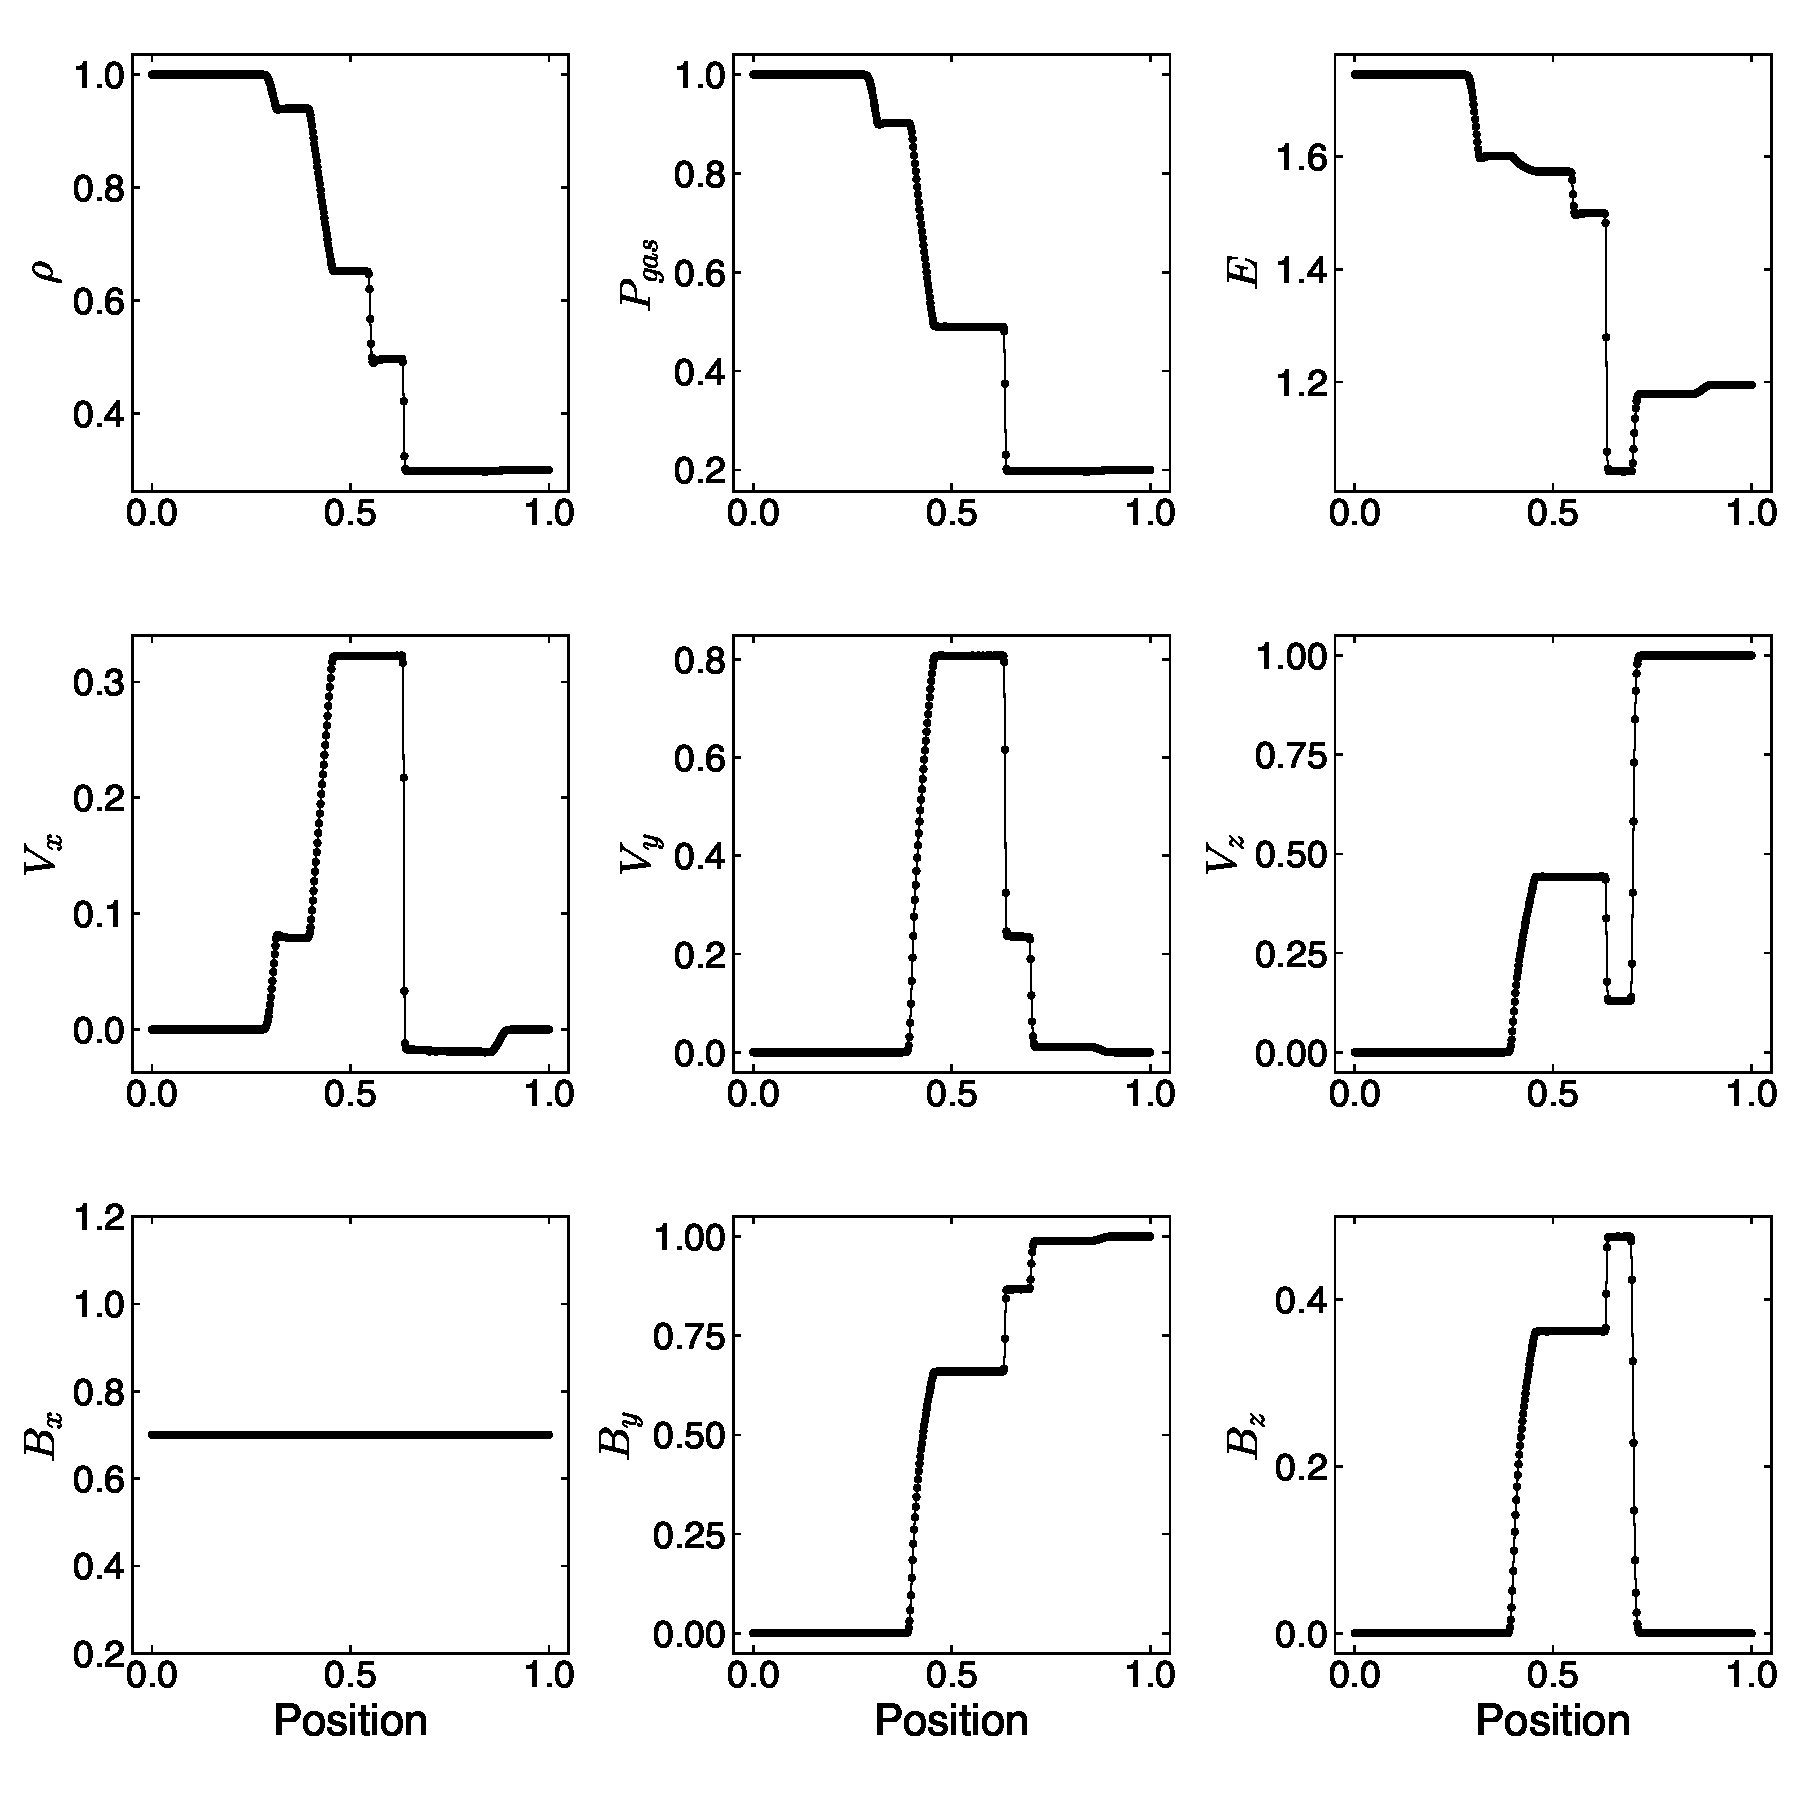
\includegraphics[width=\linewidth]{assets/3-mhd-tests/rj4d.pdf}
    \caption{Ryu \& Jones 4d Shock Tube solution \citep{ryu_jones_1995}.
    \input{|python ../python/get_links.py 'rj4d'}}
    \label{fig:rj-4d}
\end{figure}

\paragraph{MHD Einfeldt Strong Rarefaction}

The MHD Einfeldt Strong Rarefaction test \citep{einfeldt_1991} creates a strong outflow and central vacuum state. The diverging solution leads to an extremely strong and fast rarefaction where the energy is dominated by kinetic energy and as such can often reveal challenges for finite-volume methods with near-vacuum states, since some Riemann solvers will return unphysical solutions with negative density or negative internal energy. High values of the outflow velocity ($V_{out}\ge3$) can also lead to spurious oscillations in the solution. $V_{out} = 2$ was chosen for this test \citep{charm_2011}.

\begin{figure}[ht!]
    % \epsscale{0.5}
    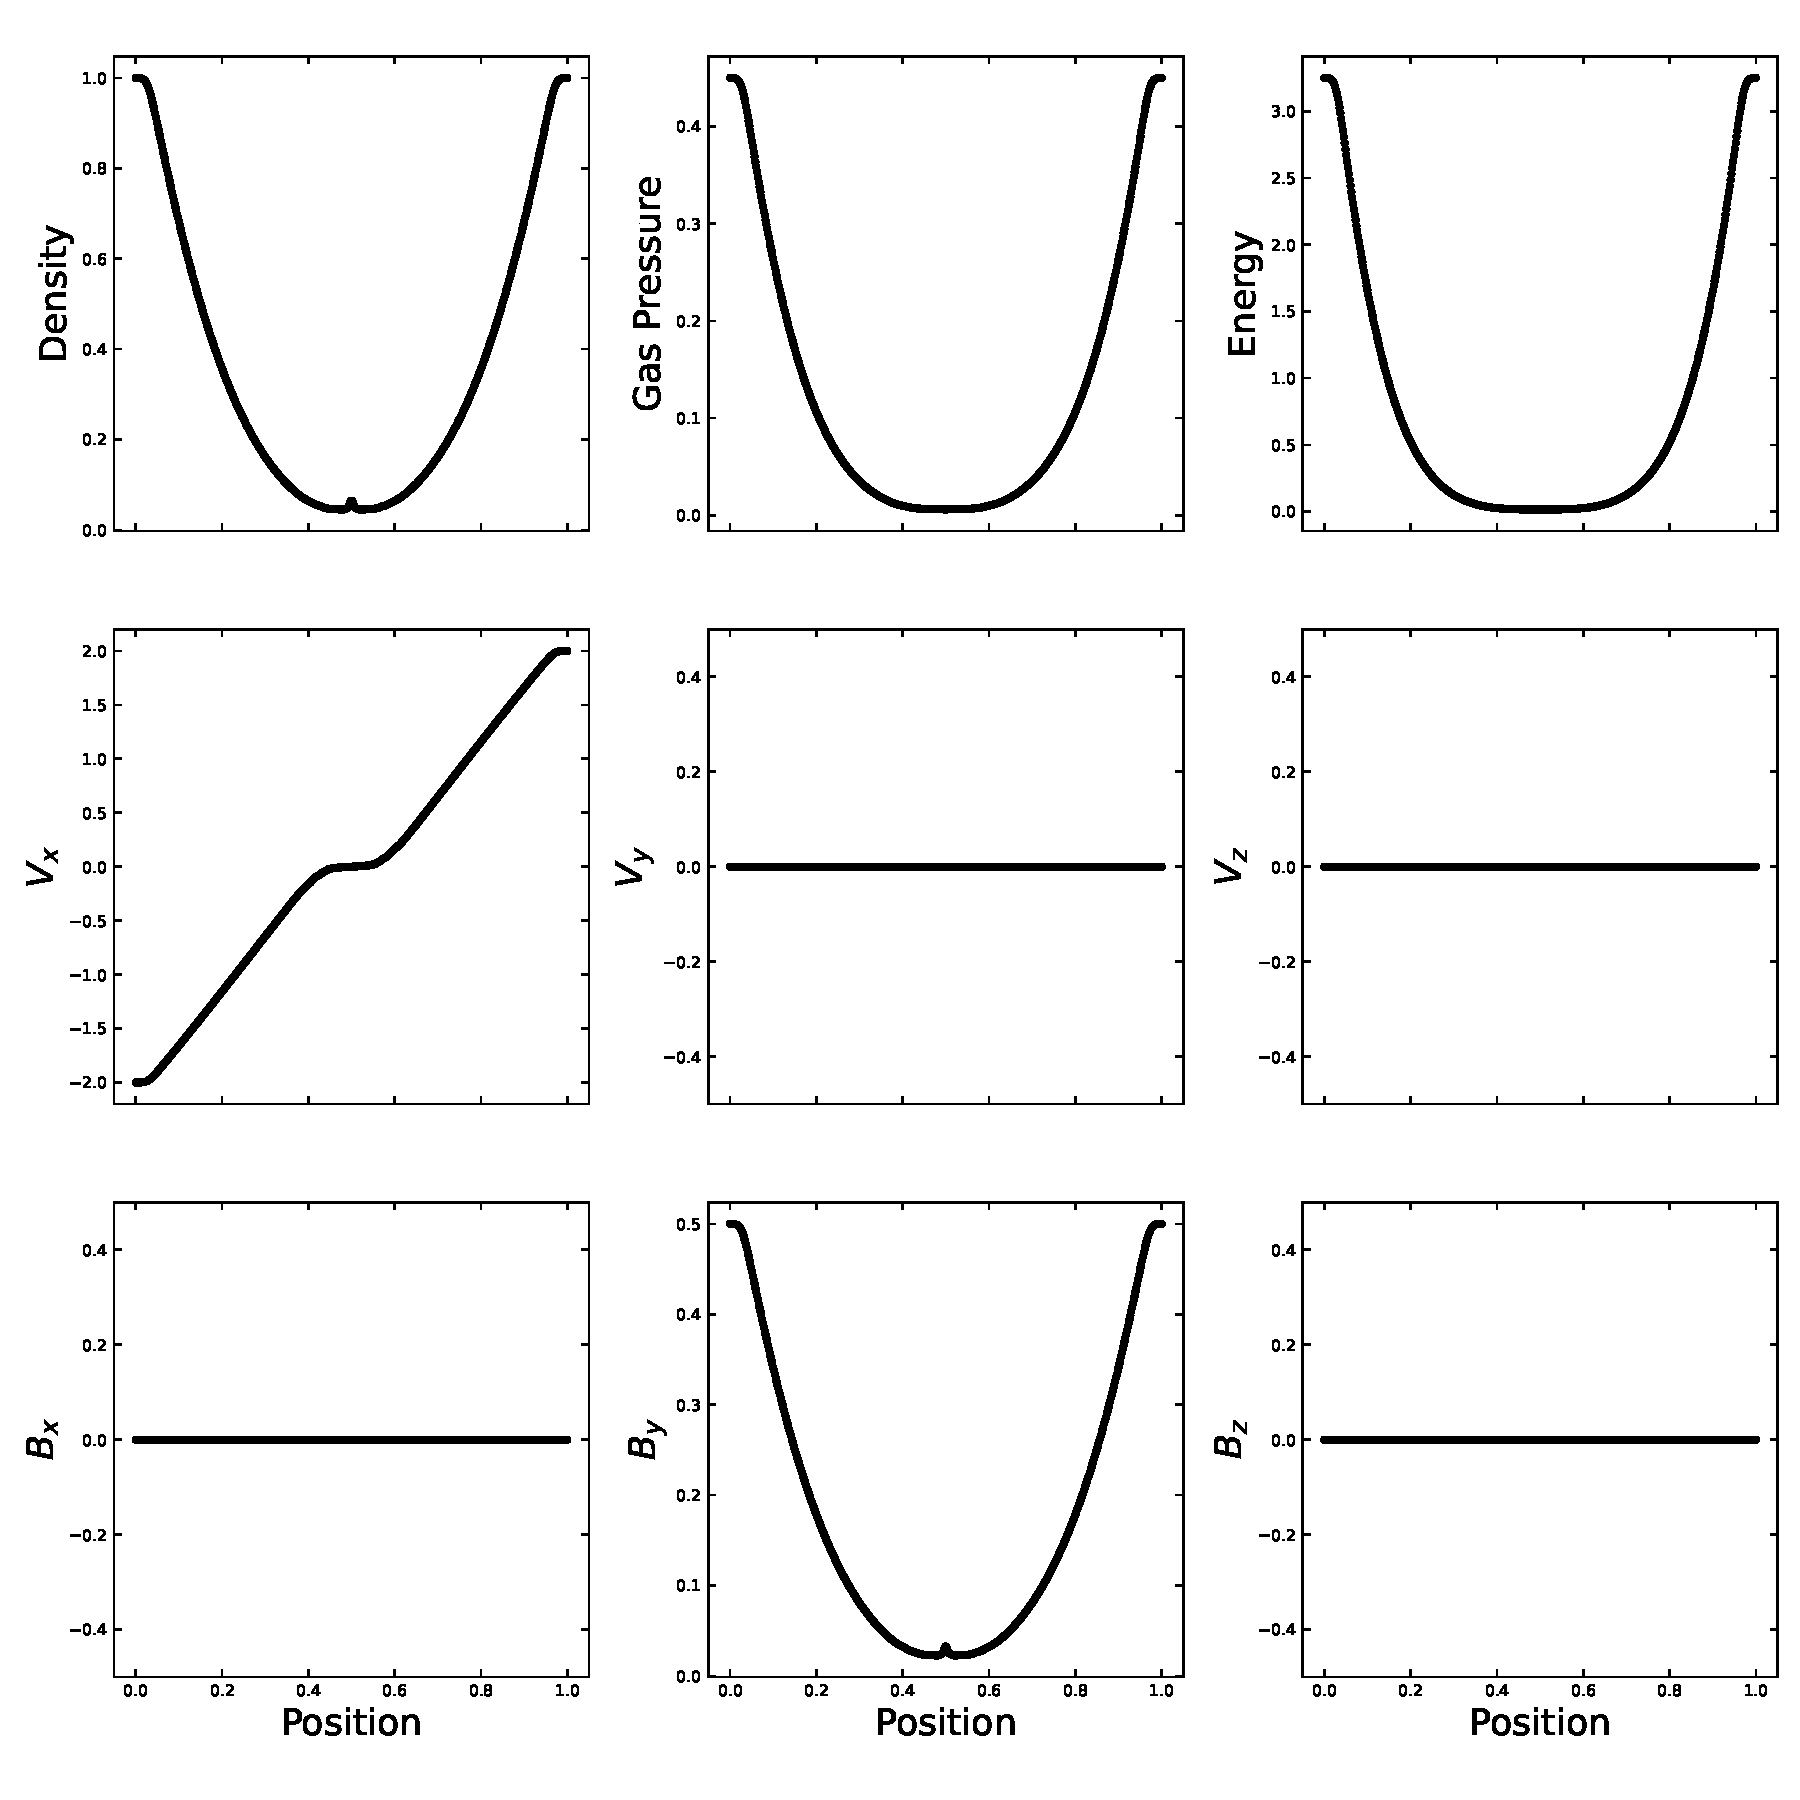
\includegraphics[width=\linewidth]{assets/3-mhd-tests/einfeldt.pdf}
    \caption{MHD Einfeldt Strong Rarefaction solution \citep{einfeldt_1991}.
    \input{|python ../python/get_links.py 'einfeldt'}}
    \label{fig:einfeldt}
\end{figure}